\chapter{MAD-F Development}
\label{chapter:Chapter 4}
\lhead{Chapter 4. \emph{MAD-F Development}}

In this Chapter, we present the development steps towards the implementation of the \emph{Modular Anomaly Detection Framework} MAD-F. Firstly, we present a list of the technologies used in this work. Then we undertake a data analysis from a historical AIS data-set. And finally, the implementation of each MAD-F module is individually  explained, providing a detailed clarification of the undertaken approaches.

%used methods detailing the technologies used, and methods for each developed module.

In order not to develop a fully static framework, a modular development was applied instead. This allows specific modules of the framework to be instanced multiple times with different configuration; or even the possibility of having the new modules added to the framework in the future.
%As working with project, the  that a future work could be developed based on this work, as either single modules can used, or new modules can be added to the MAD-F. 

For this end the choice of technologies was done by by emphasising efficiency handling large quantities of data and scalability. Implementation of this Framework was done with the programming language Python, using different specific packages for the different specific tasks. The used packages and their usage will be explained throughout this Chapter. Architecturally wise, the framework was implementing following an somehow layered architecture, similar to the \emph{Lambda Architecture}, which was firstly introduced by the authors in \cite{Marz2015BigSystems}. As so, the chosen data-base for this framework was Apache Cassandra \footnote{http://cassandra.apache.org/}, which was essential to store the aggregated $BPs$ in a fast and effective way. The detailed usage of the data-base is explained in \ref{section: 4 Unsupervised Trajectory Extraction}. The reception of $BPs$ by the \emph{Unsupervised Trajectory Extraction} module was done using a message queue system Apache Kafka \footnote{https://kafka.apache.org/}. The same message queuing approach as also implemented for the modules who needed to send and consume messages between them. A detailed explanation of such implementation is provided in the following sections.

\section{Data Analysis}
\label{section: Data Analysis}
In order to gain insight and find the limitations of the AIS data, our initial step towards the implementation of the framework was a the analysis of an historical AIS data-set. The analysed Data-Set was compiled, and made publicly available by another H2020 European Project\footnote{http://datacron-project.eu}. 
This data-set was chosen, due to the completeness of documentation and description of the actual data-set; which to the extend of our knowledge was the only open-source AIS data-set with such characteristics.  

In this Section, we present a data analysis from the data-set \cite{DATASET}. We conducted this data analysis, by firstly providing a general description of the used data-set, and secondly by analysing the overall feature distribution of the each feature in the used data-set.
The used data-set, is composed from \textbf{18.684.115} AIS messages originated by \textbf{4555} different vessels. The Data-Set covers a Period of 6 Months (from 2015-10-01 to 2016-03-31), from a area nearby Brest, France as it is presented under in Figure \ref{fig:DS_Sample}.

\begin{figure}[H]
\centering
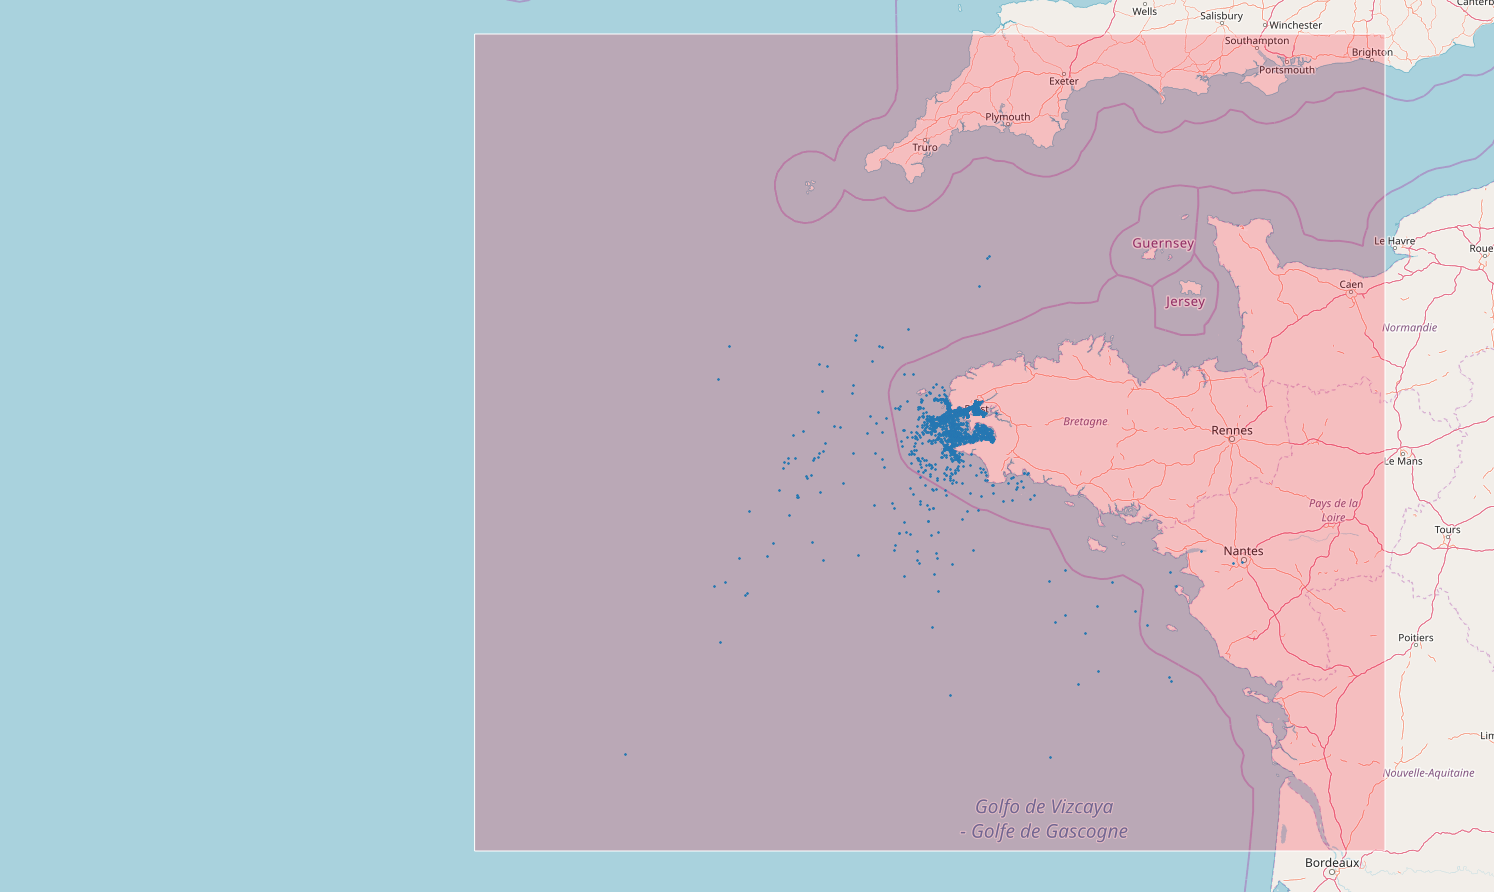
\includegraphics[scale = .23]{figures/Ch4/nari_DS_ex2.png}
\caption{Area of the Data-Set represented in the Red, with a sample of 50.000 AIS Positions.}
\label{fig:DS_Sample}
\end{figure}

Every AIS message provided in the data-set, is composed by the features that derive from the AIS dynamic information. In Table \ref{Table: Data-Set Features}, we describe the data-set features by detailing their units and their unit range. 

\begin{table}[H]
\centering
\caption{AIS dynamic messages features description.}
\label{Table: Data-Set Features}
\begin{tabular}{@{}llll@{}}
\toprule
Feature & Description                  & Unit               & Range          \\ \midrule
MMSI    & Vessel Unique Identifier.     &                    & 0 to 99999     \\
Status  & AIS Navigational Status.     &                    & 0 to 15        \\
Turn    & Rate of turn, right or left. & degrees per minute & 0 to 720       \\
SOG     & Speed Over Ground.           & knots              & 0 to 111*      \\
COG     & Course Over Ground.          & degrees            & 0º to 360º     \\
X       & Longitude.                   & degrees            & -180º to +180º \\
Y       & Latitude.                    & degrees            & -90º to 90º    \\
Time    & Received Time-Stamp.         & Unix Time          &                \\ \bottomrule
\end{tabular}
\end{table}

The data-set not only contains the AIS dynamic information correspondent, but also, in separate files the related vessel static information of each vessel which has reported in data-set. By interpolating the MMSI reported in every AIS message, we were able to enrich each AIS dynamic message (or row of the data-set), with the static information related to the vessel which has produced the dynamic message. The vessel's static information contain information of the vessel's actual dimensions and type. The use of information related to the vessels characteristics is used in different types of behavioural analysis. In this work we used the vessel type as an key aggregation indicator, better described in Section \ref{subsection: Vessel Type}.

\section{Data Ingestion}
Data Ingestion refers to the model, where the Data is input into the Framework. As mentioned in Chapter \ref{chapter:Chapter 3}, for this work was assumed that the incoming data would be able to come in two different typologies, either from batches of AIS data or Live NMEA streams. 

Historical batches of AIS data (or data-sets), are uploaded to this module via .csv files, which then are transformed into DataFrames using the Pandas\footnote{https://pandas.pydata.org}. For each imported batch of data, the features names must be pointed to the format we present in \ref{subsection: Behavioural Point}
Although for the NMEA Streams the as the decoding of such streams was needed. The choice of methods to process and decode was not has trivial. As NMEA messages are received in high frequencies, the method to such streams into comprehensible AIS like data, needed to be stable and efficient. In order to achieve this, we used the python library libais\footnote{https://github.com/schwehr/libais}, which is implemented in the programming language C++, allowing a really efficient decoding of the incoming NMEA messages. 

In Chapter \ref{chapter:Chapter 3}, we have identified two problems that occur when working with AIS real live. In order to mitigate the duplicated reception, each received messages is tagged with a unique identifier (UUID). For this present work, the created UUID will be done by considering the ID of the vessel(MMSI), and the time the received message was generated by the vessel. Thus, if two same UUID messages are received, we the second messages is discarded, and only the first received messages is considered.

The Framework was developed to be scalable, being able to handle different sources of AIS data, although for the purpose of this work, we limited the used Data to two main sources of Data. The Data-Set presented in Section \ref{section: Data Analysis}, and the NMEA feeds made available by the Portuguese Navy.


\section{Data Pre-processing}
Data Pre-processing, represents the module that handles the raw/unprocessed AIS data, Cleaning, Transforms and Normalises every AIS messages, coming from the Data Ingestion Module. Every AIS message is transformed into our normalised representation of and AIS message, which we defined as a \textbf{Behavioural Point}, defined under in \ref{subsection: Behavioural Point}.

\subsection{Latitude Longitude Normalisation}
In order to normalise the reported vessels positions, either from the AIS streams or the used Data-Set, we defined a set number of decimal cases used. This is done as most of AIS providers only assure a GPS precision of 0.0001 minutes accuracy, but what we found was that some reported positions come with up to 8 decimal cases, which can be caused just from how the Data-Set files were written.

So our normalisation process, was to assure that every vessel position was normalised to a precision on 4 decimal cases; as it represents a global position precision of 11m to 4m, as it is shown in Table \ref{Table: Degree Precision}.

\begin{table}[H]
\centering
\caption{Degree precision versus the approximate radius of measured error.}
\label{Table: Degree Precision}
\begin{tabular}{lrrrr}
\hline
\multicolumn{1}{c}{\begin{tabular}[c]{@{}c@{}}Decimal \\ Places\end{tabular}} & \multicolumn{1}{c}{Degrees} & \multicolumn{1}{c}{\begin{tabular}[c]{@{}c@{}}Precision \\ Equator\end{tabular}} & \multicolumn{1}{c}{\begin{tabular}[c]{@{}c@{}}Precision \\ 45º N/S\end{tabular}} & \multicolumn{1}{c}{\begin{tabular}[c]{@{}c@{}}Precision \\ 67º N/S\end{tabular}} \\ \hline
0 & 1.0 & 111.3Km & 78.7Km & 43.5Km \\
1 & 0.1 & 11.3Km & 7.8Km & 4.4Km \\
2 & 0.01 & 1.13Km & 787.1m & 435m \\
3 & 0.001 & 111.3m & 78.7m & 43.5m \\
4 & 0.0001 & 11.3m & 7.8m & 4.4m \\
5 & 0.00001 & 1.3m & 0.7m & 0.4m \\ \hline
\end{tabular}
\end{table}
%\todo[inline]{Geohash - https://en.wikipedia.org/wiki/Geohash}

\subsection{Data Cleansing}
Data Cleaning refers to the process of cleaning the data which is wrongly defined or, has wrong types. When handling with sensor generated data is common that wrong sensor reading can occur. In AIS data, this errors tend to occur as AIS features that are not transmitted at all, or that are transmitted with values that don't correspond to the Feature value range. An example of this is having a Latitude being broadcast with values of 500.
Therefore, we discarded all AIS messages with reported features that were not inside the feature value range. The features value range considered for the proposed framework was the one presented in \ref{Table: Data-Set Features}, which is the similar as the one presented by the authors in~\cite{Tu2016}, as the AIS default feature range.

\subsection{Behavioural Point}
\label{subsection: Behavioural Point}
Behavioural Point for this work, is our normalised feature representation of incoming vessel data. A $BP$ is a multidimensional point which is identified by the vessel id who produced the reported message. Therfore a $BP_{MMSI}$ can be represented as:

\[BP_{MMSI} = [t, x, y, SoG, CoG, NS]\]
\todo[inline]{HAVE REFS MISSING TRY TO FIND!!!}
Where the dimensions of the multidimensional $BP$ represents the features (Time, Longitude, Latitude, Speed Over Ground, Course Over Ground and Navigational Status) respectively.
Each $BP$ was correlated to one(one to one) identifier. The used identifier for this work was the Maritime Mobile Service Identity (MMSI). This choice represents certain problems, as it is mentioned by the author in XX and further discussed in Experiment XX (Section XX). Although, the non replication of the MMSI by different vessel was assumed for work. As this problem can be solved by the AIS provider, thus not occurring with every AIS provider. 
Each $BP$, as described above is further enriched by extrapolating three additional features, making each $BP$ to be represented as:

\[BP_{MMSI} = [t, x, y, SoG, CoG, NS, VT, DtS, DtP, PN]\]

Where the additional features \emph{VT, DtS, DtP, PN} representing the vessel Type, Distance to Port, Distance to Shore, Port Name. These features are not reported from every AIS messages and need to be extrapolated afterwards. The methods used to extrapolated this features are presented under Section~\ref{section: 4 Feature Engineering}. 

\section{Feature Engineering}
\label{section: 4 Feature Engineering}

\subsection{Vessel Type}
\label{subsection: Vessel Type}
Vessel Type, is a classification system, where each vessel is categorised by the type of activities it preforms. Classified by a numeric scale from 0 to 99. The first digit represents the general activity category of the vessel, and the combination of the first digit with the second represent the specific activity of the vessel. In Table~\ref{Table: Vessel Type Description} we list all the general vessel categories which are associated with the first digit of the vessel type feature, but also we present the specific vessel categories for the more frequent vessel types occurring on the data-set.

\begin{table}[H]
\centering
\caption{Vessel Type categorisation and most frequent representation.}
\label{Table: Vessel Type Description}
\begin{tabular}{@{}clll@{}}
\toprule
First Digit & General Category                                        & Relevant Categories                                        &                                                                                         \\ \midrule
1           & Reserved                                                &                                                            &                                                                                         \\
2           & Wing In Ground                                          &                                                            &                                                                                         \\
3           & Special Category                                        & 30 - Fishing                                               & 30 - 286(6\%)                                                                           \\
4           & High-Speed Craft                                        &                                                            &                                                                                         \\
5           & Special Category                                        &                                                            &                                                                                         \\
6           & Passenger                                               &                                                            &                                                                                         \\
7           & \begin{tabular}[c]{@{}l@{}}Cargo\\  \\  \end{tabular} & \begin{tabular}[c]{@{}l@{}}70 - Cargo\\ \\ \end{tabular} & \begin{tabular}[c]{@{}l@{}}70 - 1511(33\%)\\ 79 - 273(6\%)\\ 71 - 217(5\%)\end{tabular} \\
8           & Tanker                                                  & 80 - Tanker                                                & 80 - 342(7\%)                                                                           \\
9           & Other                                                   &                                                            & 99 - 1192(26\%)                                                                         \\ \bottomrule
\end{tabular}
\end{table}

For the used Data-Set described above in Section\ref{section: Data Analysis}, the Static Vessel Information is available for all the vessel in the Data-Set. Although, when handling Real-Time NMEA streams or other Batches of Data, the Vessel Static information is not available or broadcast. This, creates a problem of not having the Vessel Type information which is used to query our Trajectory Data-Base.
For this we developed a \textbf{Web Scrapping application}, described in the following subsection.

\subsubsection{Vessel Type Scrapper}
Web Scrapping is used to extract information from freely available websites. For the sole purpose of this work, we developed an application that would retrieve the Vessel Type information from a "well known vessel traffic webpage".
By providing the vessel MMSI to the Vessel Type Scrapper, we retrieve the html webpage data that contains all the static vessel information available on the "well known vessel traffic webpage". From the html data we, striping the html tags, and the non relevant specific webpage information, we access Vessel Type, as it is presented in Fig. \ref{fig:Scraper}.

\begin{figure}[H]
\centering
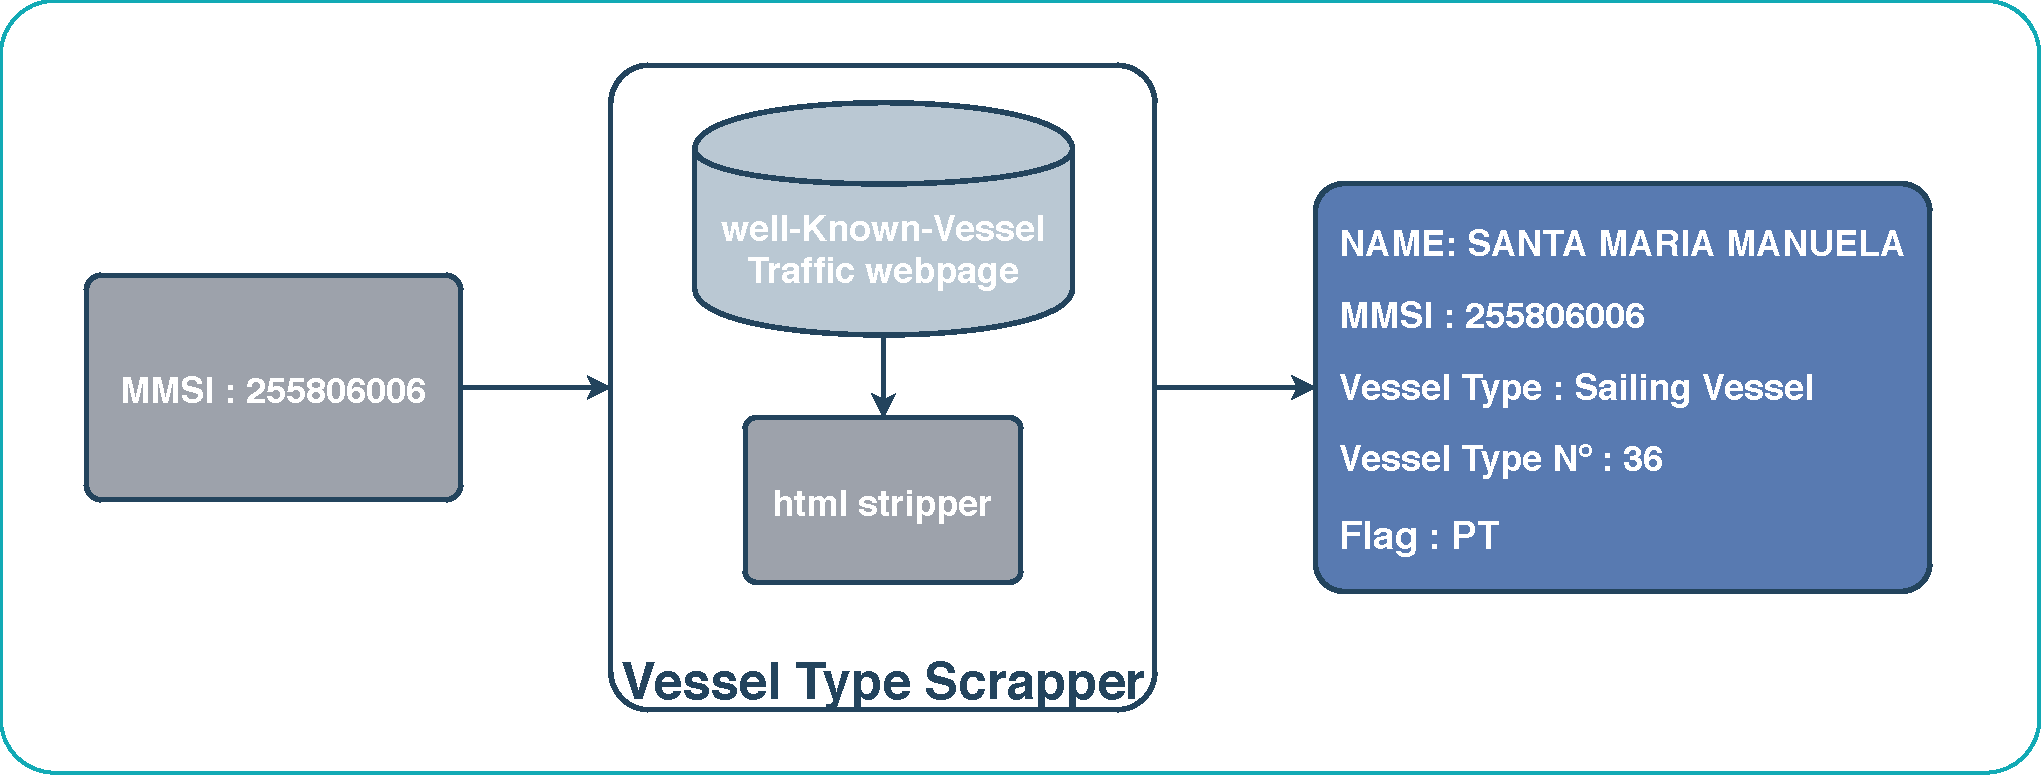
\includegraphics[scale = .4]{figures/Ch4/scrapper}
\caption{Example of the Vessel Type Scrapper retrieved information for Vessel MMSI: 255806006}
\label{fig:Scraper}
\end{figure}


\subsection{Distance to Coast}
\label{subsection: Distance to Coast}
Distance to Shore influences, the navigational behaviour for the major part of Vessel Types. In order to enrich the $BPs$ which will feed the Anomaly Detection modules, and as the distance to shore is without a doubt a valuable aggregation feature for the maritime domain. We extrapolated the Distance to Shore for every received AIS message. 

Although in order to calculate the distance to shore effectively either over historical batches of data or in real time to streams of AIS data, a efficient representation of the coastline is needed. 
For this we used the ocean coastline data\footnote{http://naturalearthdata.com}. This representation has mapped Global coastline in a vector of \textbf{547.503} points, which is equivalent having a 1:10m Global coastline representation.

The calculation of the closest point was done with a Nearest Neighbour approach, using the Ball Tree algorithm. The choice of this algorithm was done, due to the high volume of data we were using, and the possibility of using the Haversine Distance measures in the already implemented methods from \footnote{http://scikit-learn.org/stable/modules/generated/sklearn.neighbors.BallTree.html}.

Haversine is the most commonly used distance metric in the vessel navigation. As both Latitude(y) and Longitude(x) features are represented in a spherical coordinate system, the use of the most common Euclidean distance is not applicable. Thus we used the Haversine Equation \ref{eq: Haversine}, represented under.

\begin{equation}
d = 2r sin ^{-1} \sqrt{sin^2(\frac{lat_{p_2}-lat_{p_1}}{2})+cos(lat_{p_1})cos(lat_{p_2})sin^2(\frac{lon_{p_2}-lon_{p_1}}{2})}
\label{eq: Haversine}
\end{equation}

Where $d$ takes as input $({p_1}, {p_2})$, and it calculates the haversine the 2 point represented as $p1(lat_1, lon_1)$ and $p2(lat_2, lon_2)$. $r$ represents the approximate radius of the Earth which for this work we considered \textbf{6.367.000m}.

\subsubsection{Distance to Port}
Distance to Port, to the maritime scenario, and more specifically maritime international trade, represents an additional feature which is of great importance. The Estimation of Time of Arrival presents itself as a necessity for container terminals, as this terminals base operational decisions on such estimation. The estimation of time of arrival, and the prediction of the arrival port based on past vessel trajectory information, are two tasks which use the distance to port feature for such purpose, \cite{Moussa2018ScalableSpark}, \cite{Rosca2018PredictingRoutes}.

This being said, we enriched each $Behaviour Point$ by calculating the actual nearest port, and the distance to it. To achieve this, we used a similar approach as explained above in Subsection \ref{subsection: Distance to Coast}.

Although, getting a list of every port was not trivial, as there are numerous ports around the World, and such information is not 
centralised nor normalised.
We accessed the detailed information of the World Port Indexes in \footnote{http://msi.nga.mil/MSISiteContent/StaticFiles/NAV\char`_PUBS/WPI}. The World Port Index data was in a GIS(Geographic Information System) shapefile format, which is common format for the Maritime Domain, but not usable in our Framework. Therefore, we firstly normalised the data format using the Python dbfread\footnote{http://dbfread.readthedocs.io}, and then stored the normalised port data in our data-base. 
For each of the \textbf{3865} ports we extracted the respective Port position, Country, and Name. 
In Figure \ref{fig: 4 Ports} we present the port position over the Iberian coast in Orange.

\begin{figure}[H]
\centering
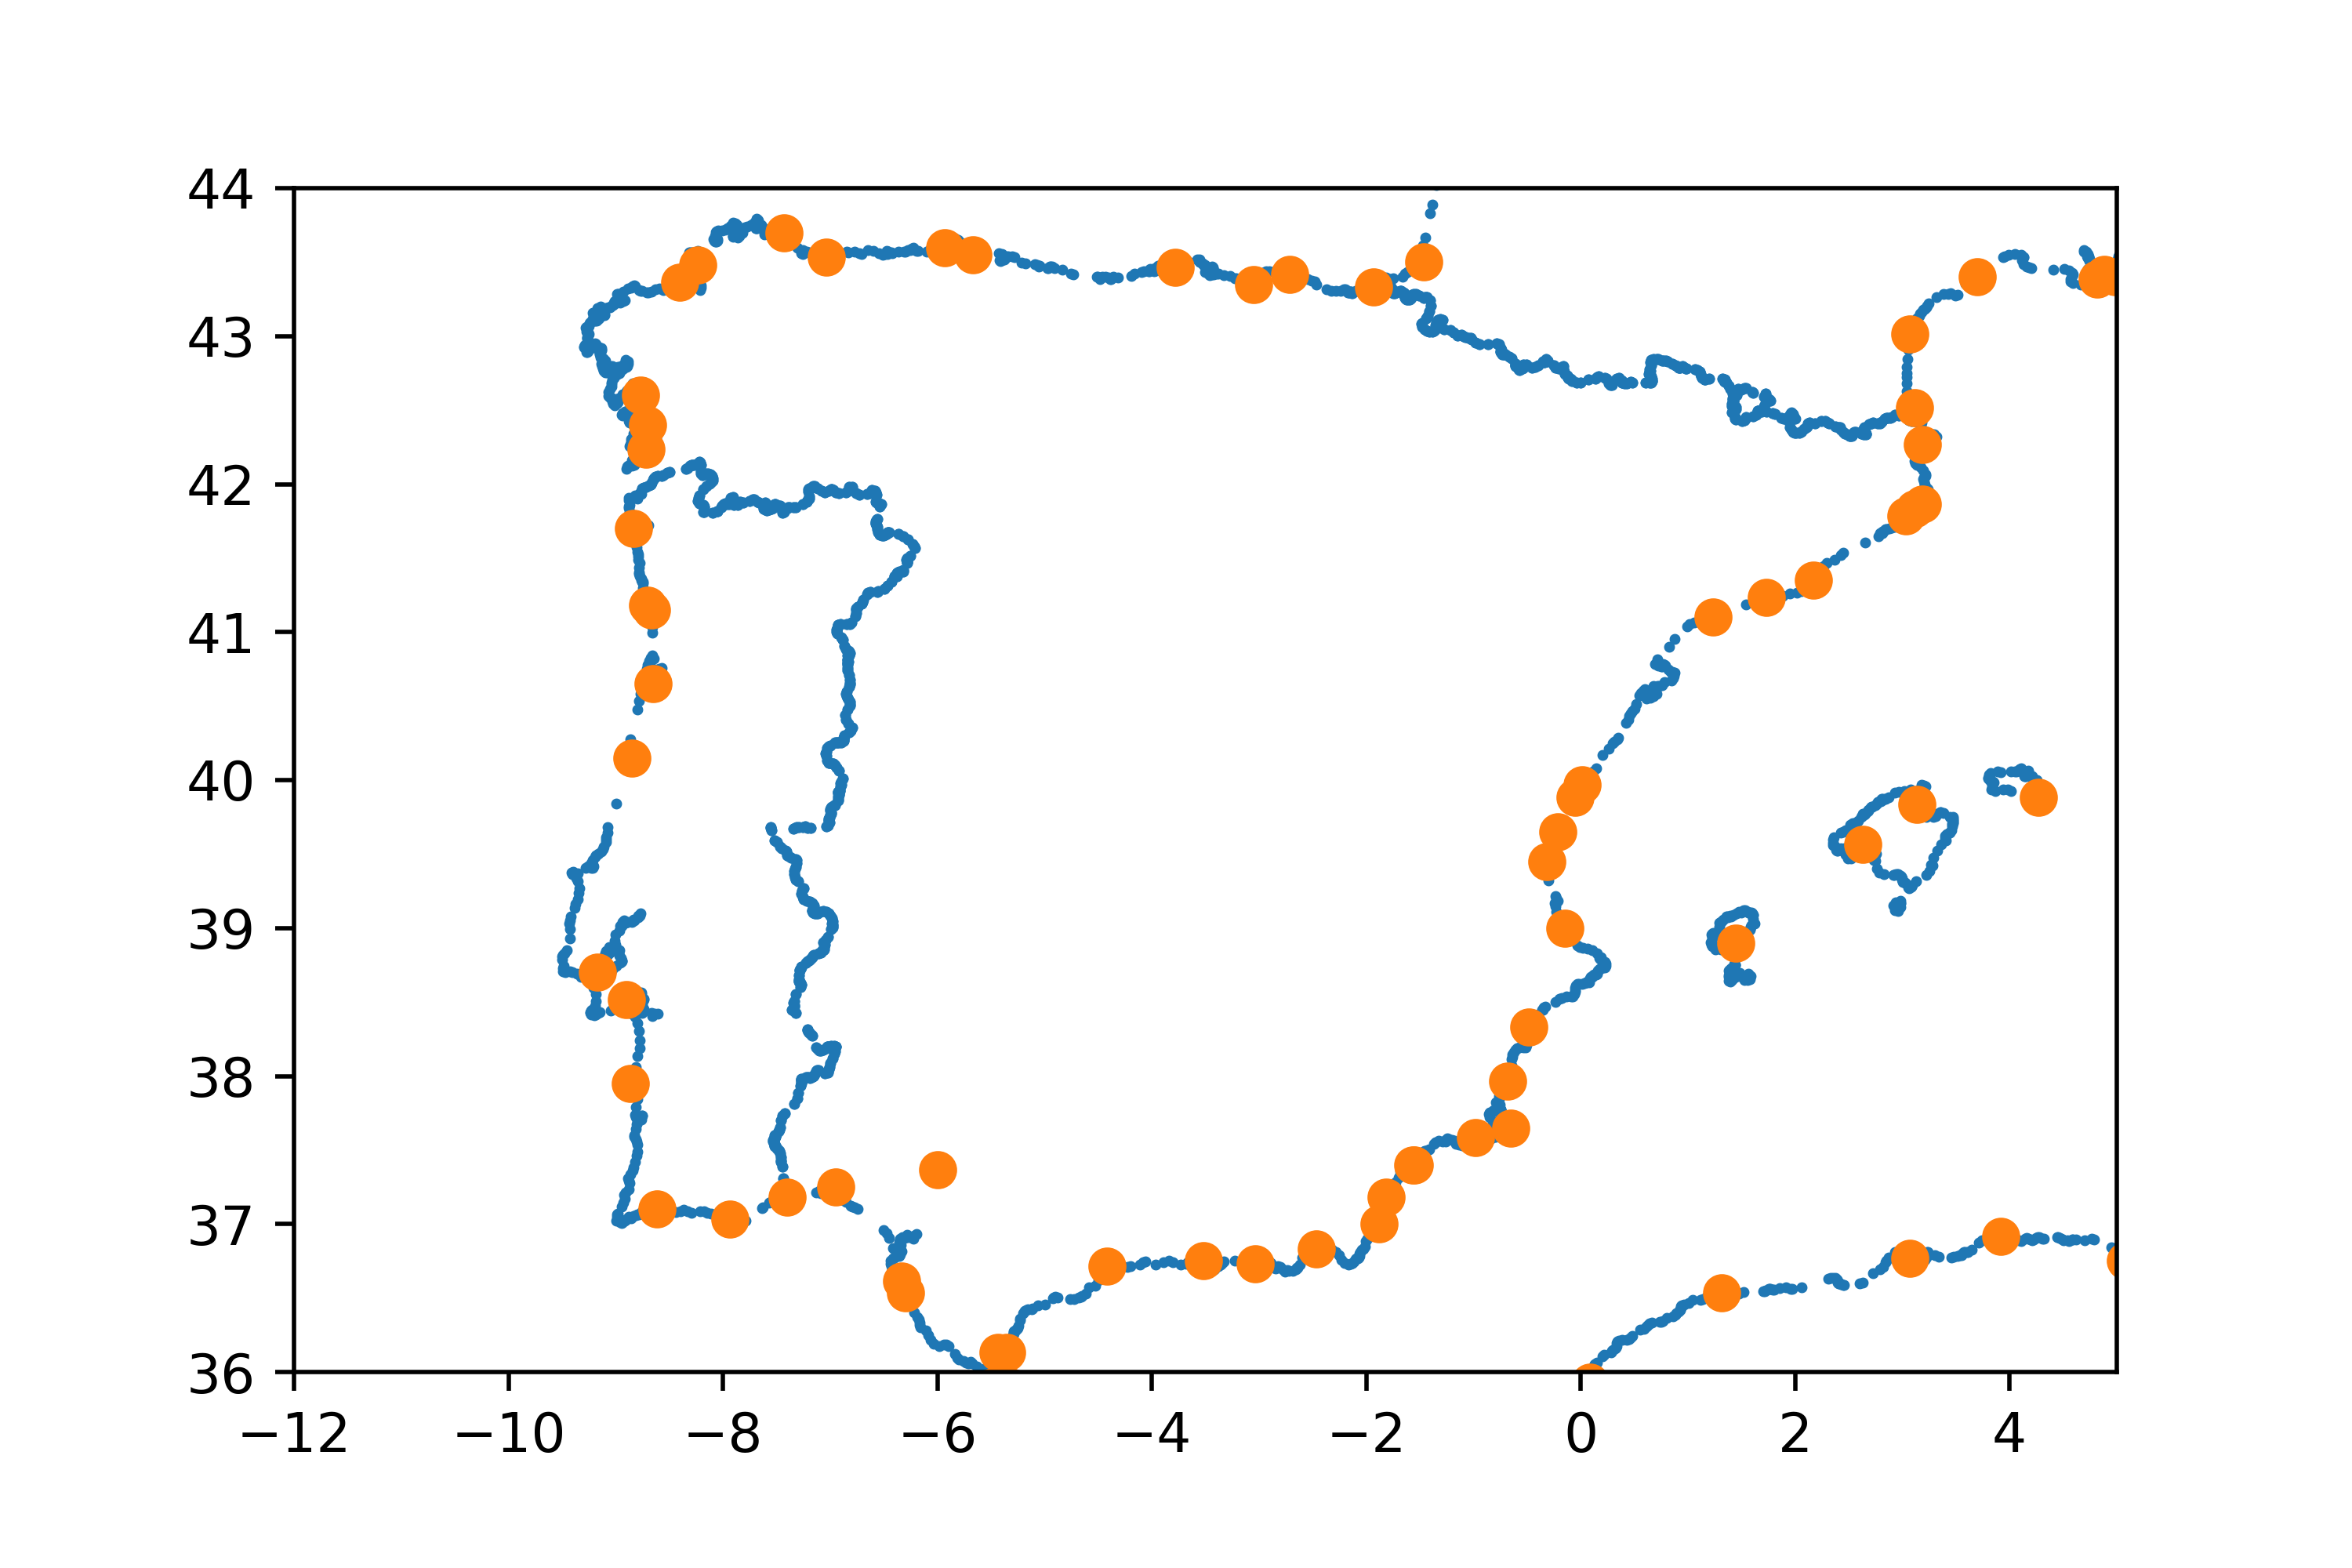
\includegraphics[scale = .9]{figures/Ch4/ports.png}
\caption{Iberian Ports(in orange), with the considered coastal Points(in Blue)}
\label{fig: 4 Ports}
\end{figure}

\subsection{Stopped/Moving}
\label{subsection: Stopped/Moving}
Enriching the reported $BPs$ by determining if at this point in time a vessel was in fact moving or stopped represents an overall information gain over the whole vessel trajectory. Such information can be used for the understanding of the normal vessels behaviour, or the detection of global points of interest.
Thus, in order to gain such information, we used two different method. The first one was a point based approach, where we infer if whether a vessel is stopped or moving based on the last report, this method is described under in this Subsection. The second approach involves the use of a vessels past trajectory information, we present this approach further in this Chapter in Section \ref{subsection: Smoothed Stopped / Moving}.

\textbf{Rule Based Approach}:
This approach is vastly used in the literature, as it is the simplest way to characterise the stopping of a vessel, based solely on the vessels reported speed or as reported by the AIS the Speed Over Ground (SOG). Thus, a $BP$ which has a reported speed under a certain defined threshold $\Delta$ is considered as stopped and the opposite are considered moving. As it is shown in equation \ref{eq: MovingRule}, where $BP_n$ represents actual Behavioural Point we want extrapolate the stopped or moving feature.

\begin{equation}
kinematic status(p_n) = \left\{\begin{matrix}
BP_n.SOG > \Delta; & Moving\\ 
BP_n.SOG \leq  \Delta; & Stopped
\end{matrix}\right.
\label{eq: MovingRule}
\end{equation}

The most commonly used $\Delta$ value found in literature was 0.5 knots.
This approach despite fitting most of the vessels behaviours, for the some types of fishing vessels it does not fit such behaviours. This occurs as some fishing activities, require the vessel to be drastically slow down for short periods of time.
In Figure~\ref{fig: 228858000}, we present a fishing vessel trajectory, where points represented in blue are considered as stopped points.   

\begin{figure}[H]
\centering
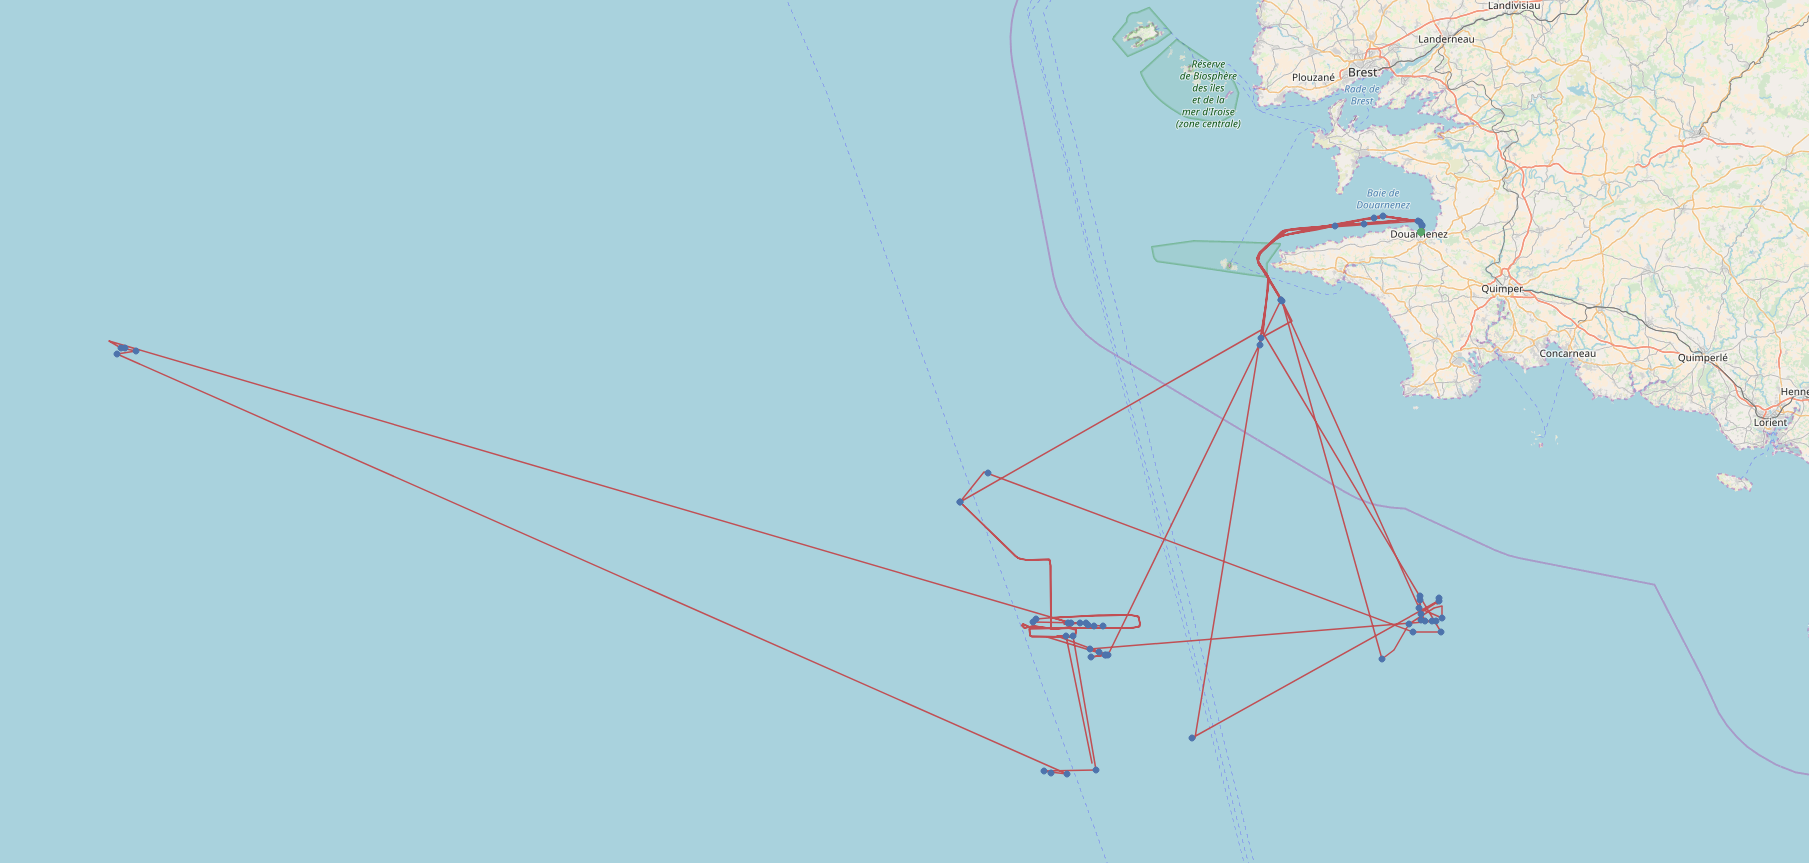
\includegraphics[scale = 0.2]{figures/Ch4/simplestopMoving228858000.png}
\caption{Fishing vessel 228858000 trajectory.}
\label{fig: 228858000}
\end{figure}

\section{Unsupervised Trajectory Extraction}
\label{section: 4 Unsupervised Trajectory Extraction}
In this Section we present our interpretation and the definition of what was for this work considered as a vessel trajectory. 

\subsection{Trajectory Definition}
\label{subsection: Trajectory Definition}
Representing a trajectory in a optimal way, can become a difficulty task in the maritime domain. Currently there are a vast number of solutions described in the literature. They, represent a trajectory differently, depending on the type of problem.

Our approach to represent a maritime trajectory, was to consider a trajectory as a whole. This is, as vessel are obliged to broadcast their AIS information in a semi-continuous rates. By normalising each broadcast by defining a \textbf{Behavioural Point}, we can aggregate each $BP$ based on the $BPs$ vessel identifier which is the vessel MMSI. Thus the aggregation of $BPs_{MMSI}$ represents for us a trajectory, which can be represented as:
\[TR_{MMSI} = BP_{MMSI_1}, BP_{MMSI_2}, BP_{MMSI_3}, BP_{MMSI_4}, \cdots , BP_{MMSI_n}\]
Every trajectory is then sorted, and kept sorted based on the Time-Stamp of each $BP_{MMSI}$. The representation of the $BPs$ over a time allows us to consider a each trajectory ($TR_{MMSI}$) as a multivariate time-series.
Each trajectory, can be then defined as a group of $N$ time-series. Where $N$ represents the number of features considered for the $BPs$ definition.

Nevertheless, what was considered as most relevant, for our definition of a trajectory was the effectiveness, and scalability of such representation. This is, the effective adding of new $BPs$ to a trajectory, and the accessing of historical trajectories in effective time. We achieved this by implementing the data-base in Cassandra. From such we defined a set of pre-defined queries to which allowed the effective access to a whole or partial trajectory, in near real time.
In Figure \ref{fig: TrajectorySMM_example} we represent an example of the vessel trajectory which was plotted over a map. 

\begin{figure}[H]
\centering
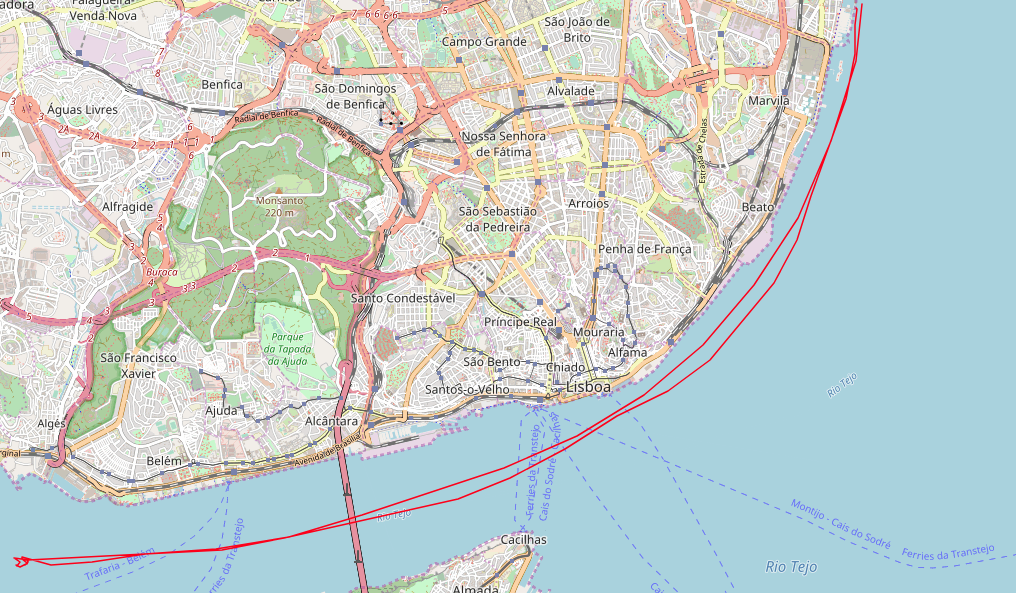
\includegraphics[width=\textwidth]{figures/Ch3/traj_example.png}
\caption{Trajectory snapshot(2017-11-05 10:22 to 2017-11-05 22:42) from Vessel MMSI: 255806006}
\label{fig: TrajectorySMM_example}
\end{figure}

The same trajectory plotted above, is also represented as a multivariate time-series, in Figure \ref{fig: MTimeSeries_example}, by just considering the four most relevant kinematic features of a $BP$, the positional features (where $x$ represents the Longitude, and $y$ represents the Latitude) and the speed and course features. 


\begin{figure}[H]
\centering
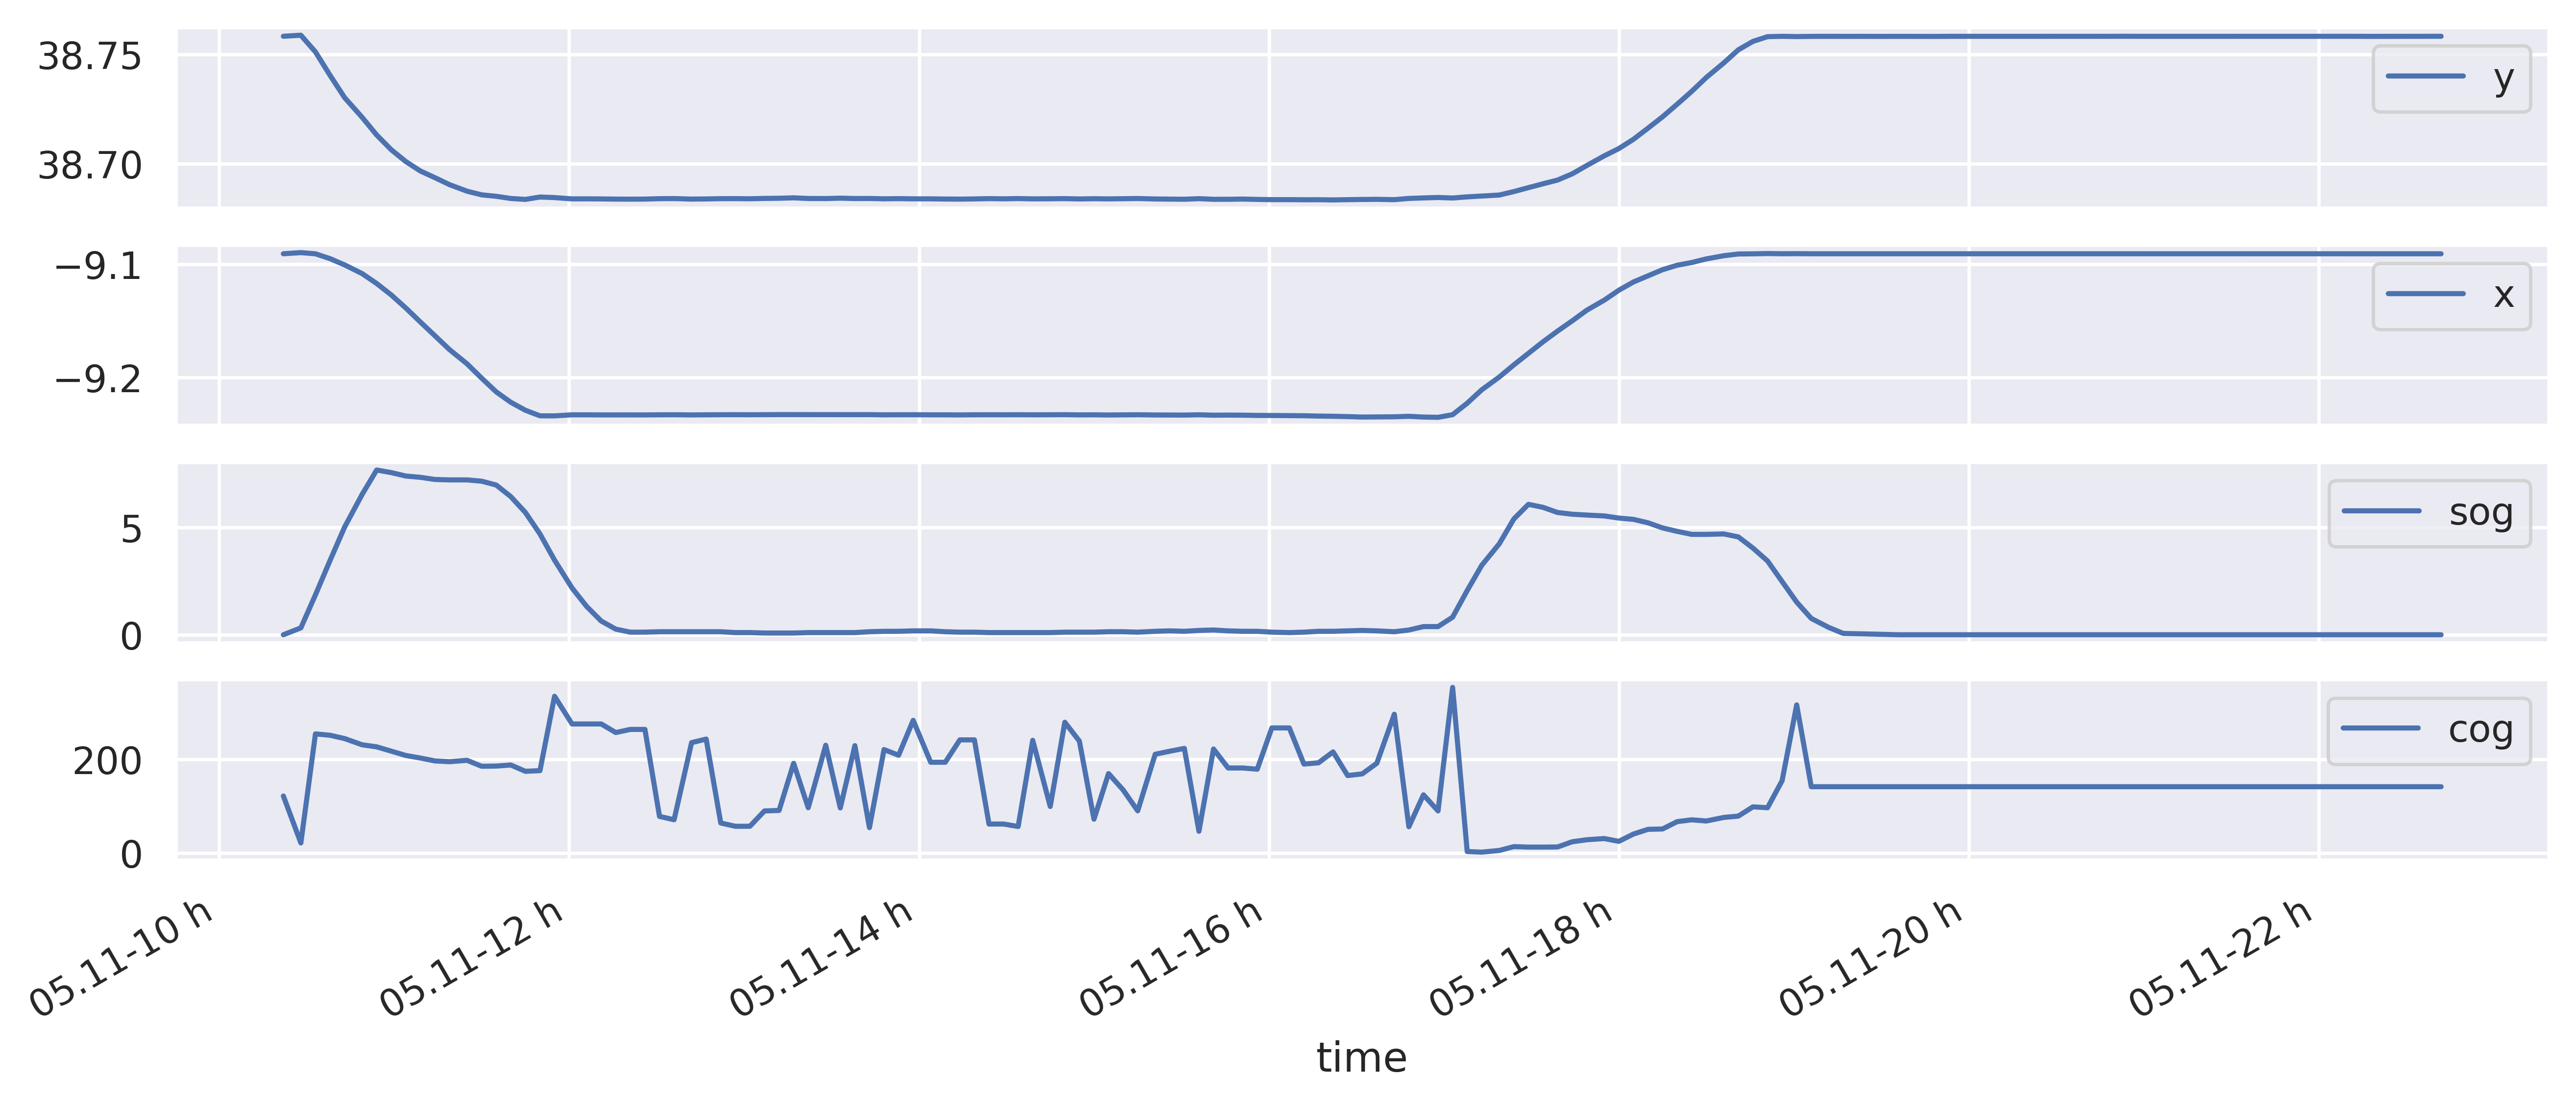
\includegraphics[width=\textwidth]{figures/Ch3/ts_example.png}
\caption{Trajectory represented in Figure \ref{fig: TrajectorySMM_example}, presented as a multivariate time-series.}
\label{fig: MTimeSeries_example}
\end{figure}

\subsection{Smoothed Stopped / Moving}
\label{subsection: Smoothed Stopped / Moving}
In order to resolve the problem presented in Section \ref{subsection: Stopped/Moving}, where the rule based stopped/moving approach had problems when dealing with some type of fishing activity trajectories. 
And also as a trajectory could be overseen as a multivariate time-series. We used a commonly used time-series analysis technique, \emph{Rolling Mean}. 
By smoothing the vessels $SoG$ time-series, based on the previous configurable $W$ $BPs$, where $W$ represent the window size considered. We smooth the random or abrupt variations in the observed speed features, which will in the end better describe the kinematic movement behaviour presented by these fishing vessels. 
The configurable $W$, allows the end-used of this framework, to configure the smoothness of the over the reported speed feature. This ultimately leads to a better representation of the vessel kinematics, which will be used for the anomaly detection methods presented in Subsection \ref{subsection: 4 Time-Space Incompatibility}, \ref{subsection: 4 Navigational Status Validation} and \ref{subsection: 4 Vessel Rendezvous}.

\begin{figure}[H]
\centering
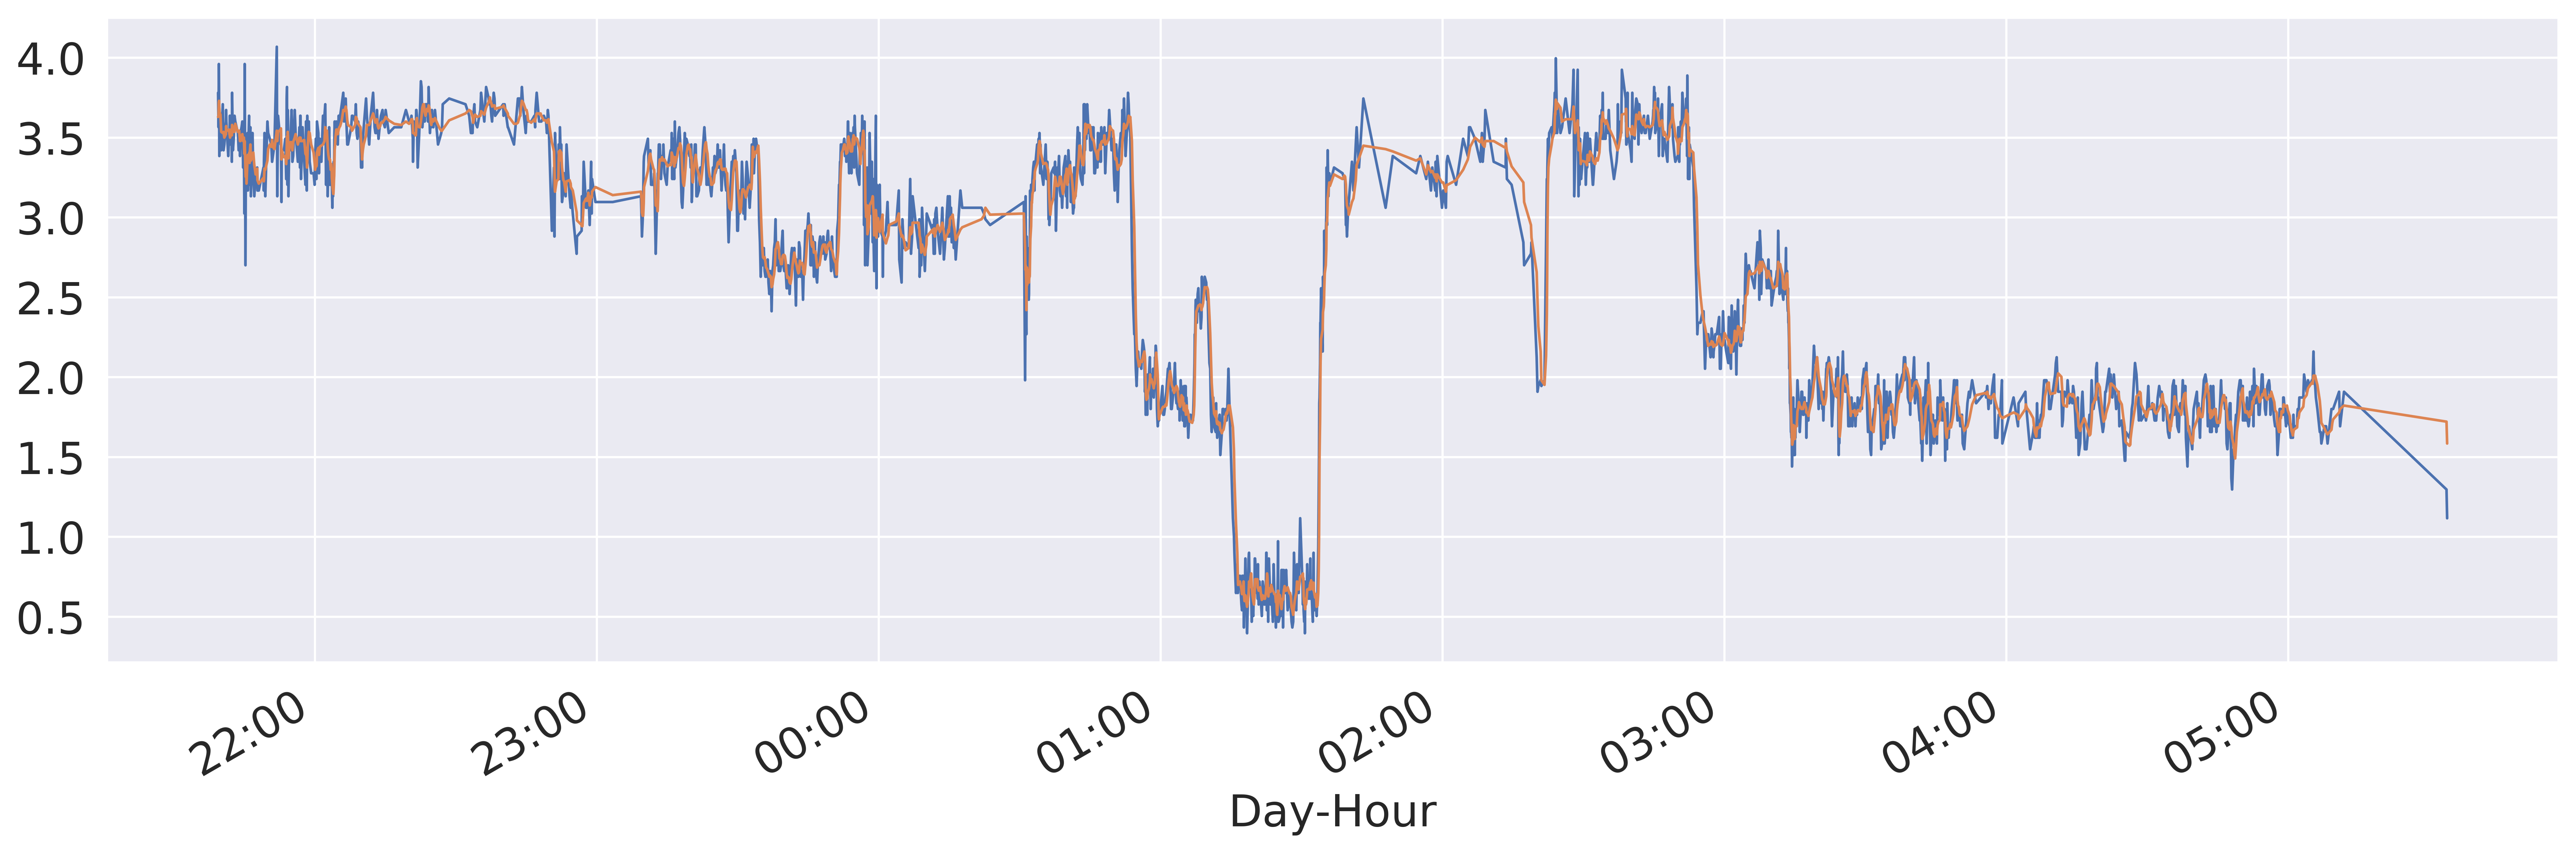
\includegraphics[width=\textwidth]{figures/Ch3/ts_smoothed.png}
\caption{Snapshot of Trajectory represented in Figure \ref{fig: 228858000} SOG feature presented as a time-series.}
\label{fig: 228858000 ts smoothed}
\end{figure}

\section{Anomaly Detection Service}
\subsection{Time-Space Incompatibility}
\label{subsection: 4 Time-Space Incompatibility}
Time Space incompatible corresponds to an anomalous or incoherent situation where the reported actual Vessels position is not compatible if compared with previous reported positions, and Vessels Kinematics. The detection of this situation, is also represented as an Anomaly Requirement \emph{$AR_4$}, in Section \ref{section: Framework Requirements}.

In order to detect this incoherence's, we developed a method that takes as input an historical vessels trajectory $TR_{MMSI}$, and for each Behavioural Point ${BP_{MMSI}}^{T-1}$ we estimate the vessels position at instance ${BP_{MMSI}}^{T}$.
The estimation is done by assuming that a vessels movement can be represented in a \emph{Linear Motion}. As vessels tend to move in the most economical way, the Vessels travelled distance, was calculated, using the formula:
\begin{equation}
Distance = Velocity . \Delta Time
\label{eq: dvt}
\end{equation}
Where $\Delta Time$ represents the actual Time Shift from point $(T-1)$ to $(T)$.

By calculating the equation \ref{eq: dvt} for each $BP^{T}$ based on the reported Position of the previous $BP^{T-1}$, we can predict that Vessel should be in a distance radius of $D$ for the next $BP^T$, as it is shown in Figure \ref{fig: dvt}.

\begin{figure}[H]
\centering
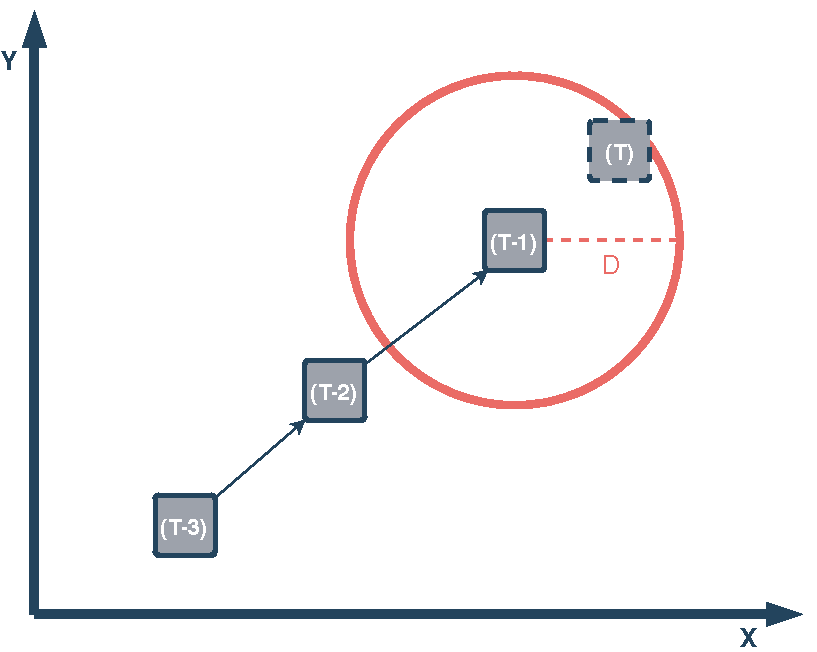
\includegraphics[scale = .6]{figures/Ch4/DVT.pdf}
\caption{Linear Estimation}
\label{fig: dvt}
\end{figure}

By defining a configurable \emph{Distance Factor Threshold} $dft$, representing a factor that would be multiplied by $D$, is possible to deduct that, if the a vessel at Time $BP^{T}$ is at a distance superior than $(D.dft)$, it is considered at a incoherent position. Therefore it is reported as anomalous.

The emphasis of this Section was on the detection of Time-Space Incompatibly, which is depend on the level of error acceptance is achieved using the methods above. 
Although by assuming that vessels have a huge inertia, making them unable to perform quick changes of speed and direction, the authors in \cite{Sadowski2015AlgorithmsCompression} present a \emph{Linear Estimation Algorithm}.
As the reported $CoG$ represents the direction of movement, it is possible to Equation \ref{eq: dvt}, thus estimating the actual position of the Vessel, opposed to the Distance from previous Position. %\todo{see if i put this here}The accurate estimation of a vessels position based on past trajectory information was left for future work. 

\subsection{Navigational Status Validation}
\label{subsection: 4 Navigational Status Validation}
AIS Navigational Status describes the vessel current activity based on a set static set of defined status, as shown in Table~\ref{Table: AIS Status}.

\begin{table}[H]
\centering
\caption{AIS Navigational Status enumeration.}
\label{Table: AIS Status}
\begin{tabular}{@{}cl@{}}
\toprule
\begin{tabular}[c]{@{}c@{}}Navigational \\ Status Value\end{tabular} & \multicolumn{1}{c}{Description} \\ \midrule
0 & under way using engine \\
1 & at anchor \\
2 & not under command \\
3 & restricted manoeuvrability \\
4 & constrained by draught \\
5 & moored \\
6 & aground \\
7 & engaged in fishing \\
8 & under way sailing \\
9 - 14 & reserved for future use \\
15 & Default \\ \bottomrule
\end{tabular}
\end{table}

The Navigational Status requires to be manually set, and constantly updated (according to the current vessel activity), by the vessel crew members.
This creates the problem of relying on Human action to update the actual vessel navigational status, which is prone to errors. 
The use of the wrong navigational status being considered an Anomaly represented as $(AR_4)$ in Section \ref{section: Framework Requirements}, our approach towards the detection of such Anomaly, started by firstly gaining insight of each navigational status, and their usage at seas.
By accessing maritime knowledge via Maritime Officers, we enriched our previous description of each navigational status, by classifying the appropriate \emph{Stopped or Moving Label} to each status. Maritime Officers based the expected kinematics of each navigational status provided the following Table \ref{Table: AIS Status Moving or Stopped}.
\begin{table}[H]
\centering
\caption{Expert stopped or moving label over the AIS navigational status.}
\label{Table: AIS Status Moving or Stopped}
\begin{tabular}{lc}
\hline
Expert Label     & Navigational Status Number \\ \hline
Stopped          & 1, 5, 6                    \\
Moving           & 0, 7*, 8                   \\
Non-Quantifiable & 2, 3, 4, 15                \\ \hline
\end{tabular}
\end{table}
$7^*$ (Engaged at Fishing) represents a special navigational status which cannot be validated with a stopped or moving analysis. Our efforts to validate this specific status are presented under in Subsection \ref{subsection: Fishing Activity Detection}.

The actual navigational status validation, is done as a \emph{point based comparison}. By comparing the previous $BPs$ enriched feature \emph{Smoothed Stopped or Moving}(Section \ref{subsection: Smoothed Stopped / Moving}) with the stopped/moving label Maritime Experts has defined for each Navigational Status.
An example for this validation could be:
If a $BP$ has been received with the Navigational Status \textit{0 - under way using engine}, but the reported Kinematics describe it as \textit{Stopped}, which for this Status should be \textit{Moving}.

\subsection{Fishing Activity Detection}
\label{subsection: Fishing Activity Detection}

Based on the Navigational Status Validation presented above we decided to enrich this methods with the detection of a special navigational status, the fishing activity (Navigational Status - 7 - Engaged in Fishing). 

Fishing is a activity that generates huge profits for the global maritime lobby. This activity being so profitable and competitive between fishing companies, generates a problem for the Maritime Authorities. To avoid informing other fishing vessel of lucrative "fishing spots", fishing vessels try to hide their location as most as possible. This behaviour is anomalous when AIS is turned off. Fishing vessels are more prone to undermine the fishing competition, leading to Illegal Unreported and Unregulated fishing \footnote{http://fao.org/iuu-fishing/en/}(IUU).  Linked to IUU is the depletion of fish stocks, as well as the destruction of marine habitats and therefore putting honest fishers at an unfair disadvantage and thus weakening coastal communities, particularly in underdeveloped countries~\cite{kroodsma2018TrackingFisheries}.

A vessel fishing activity is commonly defined as the period of time by which a vessel has fishing gear in the water. Since at the time we didn't have access to any Maritime Expert Classified data-sets, we focused on the validation of this particularly navigational status (7 - engaged in fishing) by analysing the kinematic features capable of inferring whether the vessel is currently fishing or not. 
The main characteristic that identifies the fishing activity is the fast variation of direction together with a change in the speed. This can be seen as a generalisation as there are multiple different fishing, each different one having its own specific kinematic behaviour.
Nevertheless, we claim that a fishing behaviour may be reasonably assumed to be highly dependent on speed variations. Specifically speed variations allow the fishing activity to be described by two main behavioural patterns. The first one is the \emph{high speed behaviour}, typical of a vessel steaming at normal cruising speed from a fishing spot to another. The other one, the \emph{low speed behaviour} is represented by the speed when vessels tend to drop the fishing gear in the water, or preform other manoeuvres which can be related to the fishing activity itself. Based on the work presented by the authors in ~\cite{DeSouza2016ImprovingLearning, Natale2015MappingData, Mazzarella2014DiscoveringFootprints}, this double speed behavioural profile may be represented as a bi-modal distribution of speeds. Assuming that the speed profiles are characterised by only two speed modes, it is reasonable to apply Expectation Maximisation Gaussian Mix Models in order to estimate two distribution parameters, namely the respective mean and standard deviation of each mode, and to assign the observations to one of these behavioural profiles.
Such bi-modal Gaussian distributions may be appreciated in Figure~\ref{fig: 4 gmm_example}, where a typical histogram of the distribution of the reported speed is plotted.


\begin{figure}[H]
\centering
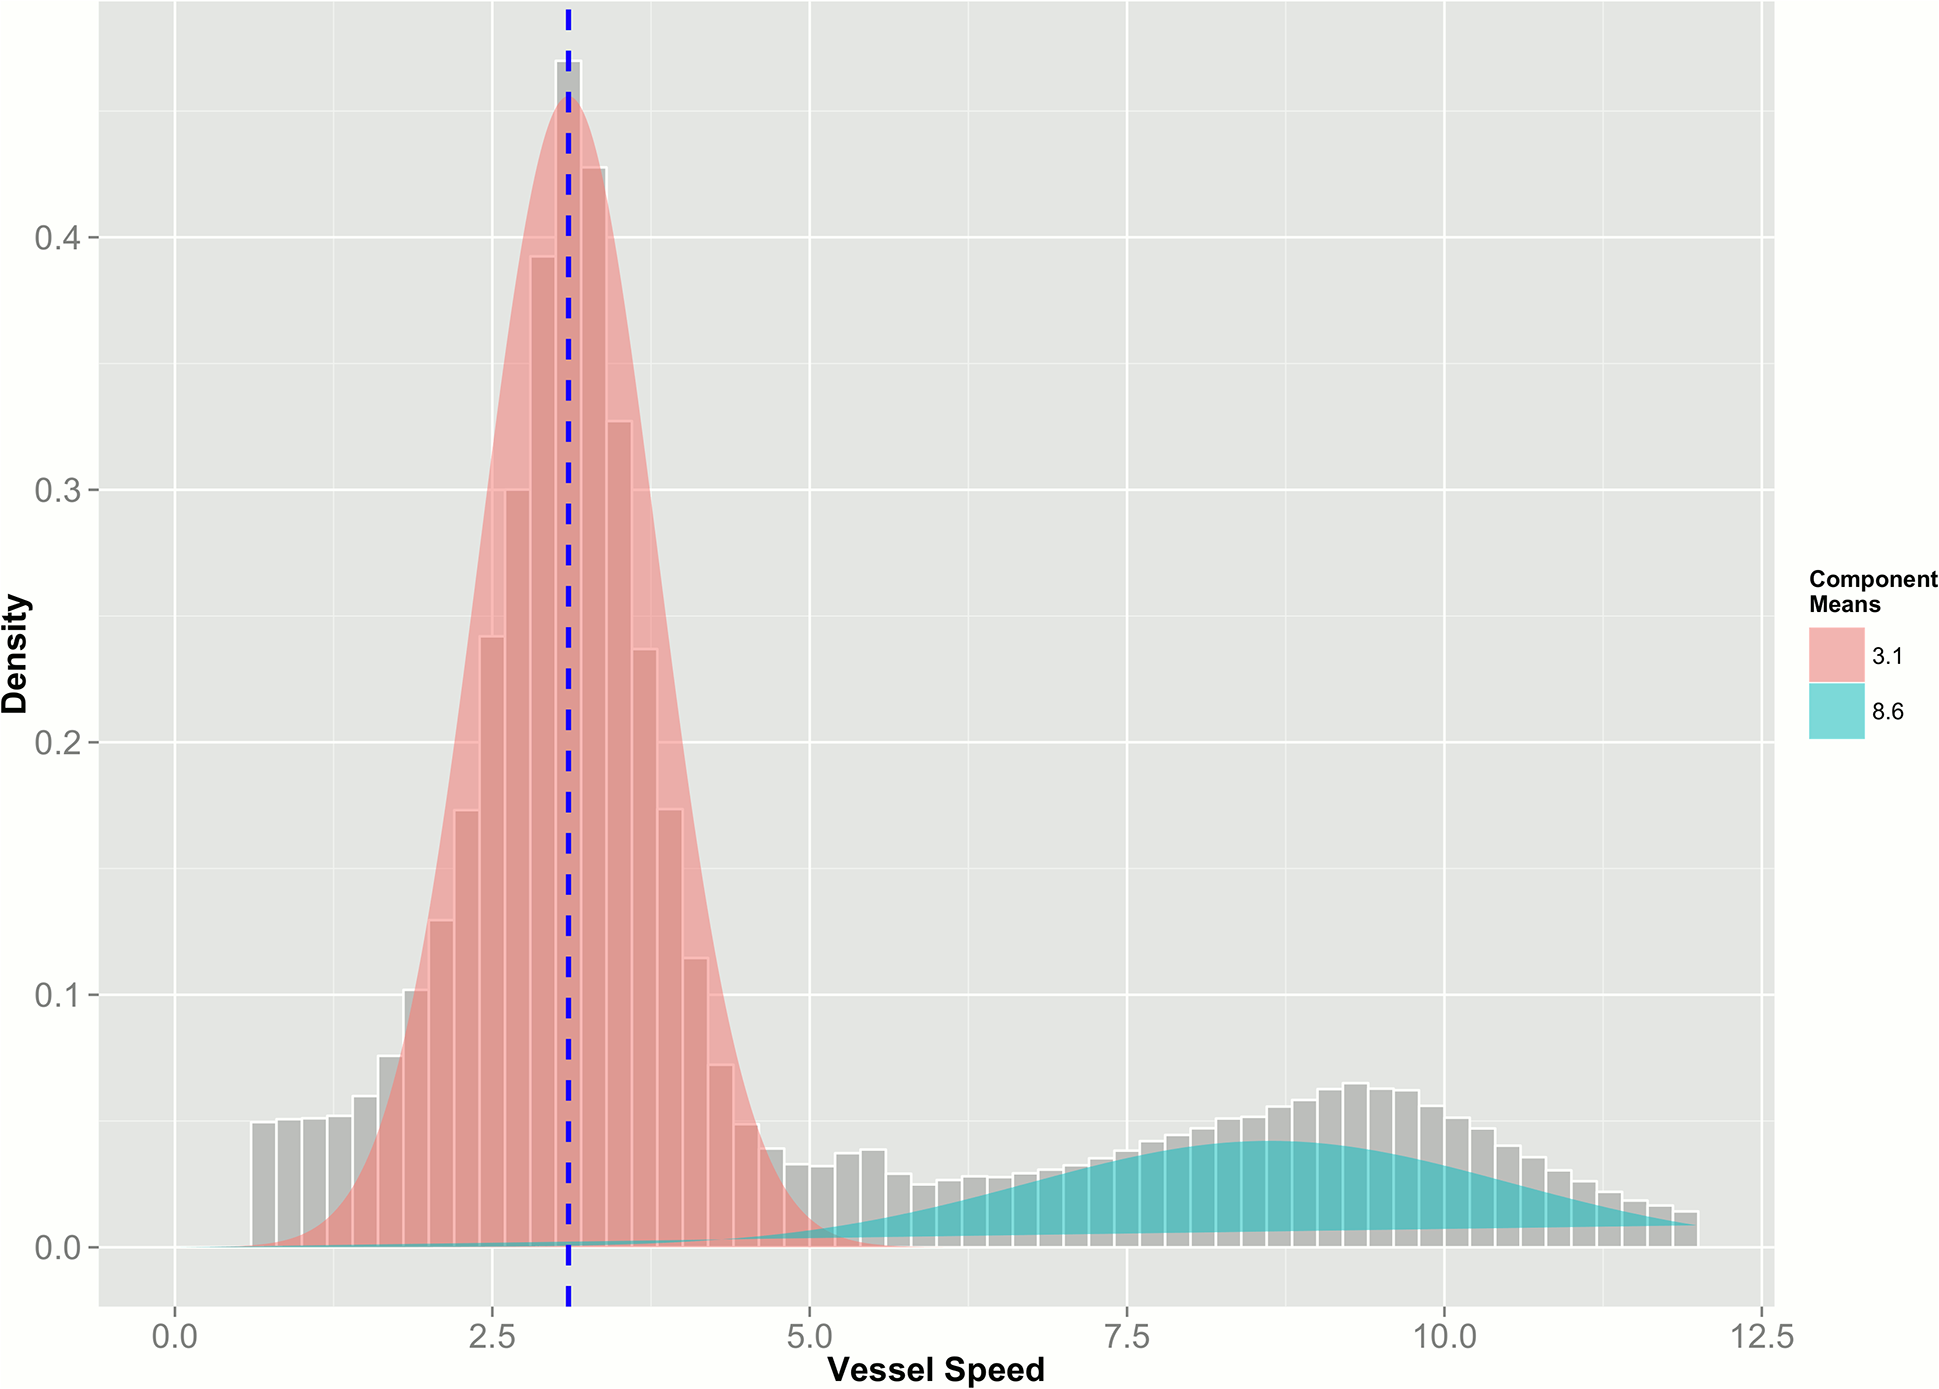
\includegraphics[scale = .7]{figures/Ch4/gmm_example.png}
\caption{Example of a XXXXXXXXXASNDLJKOANSDIKAKLOD from the }
\label{fig: 4 gmm_example}
\end{figure}

 
From the presented data-set in Section~\ref{section: Data Analysis} we fitted a Gaussian mix model to our data. This was done based on the approach presented by the authors in XX,  where we used the already developed methods of XXXrefforsklearnXXX. From the already  processed data-set, we filtered only the $BPs$ that were type Fishing Vessels (Vessel Type 30). This reduced the number of considered $BPs$ to approximately 3 Million. To avoid irregular vessel movement, and analyse the vessel movement patterns that could induce the vessel fishing activity, we filtered the $BPs$ that would be a distance of more than 2 Nautical Mile from shore, leading to a sub data-set of $436,043$ possible Fishing $BPs$.
The results and the discussion from the usage of this module are presented in Section XX.

\subsection{Vessel Rendezvous}
\label{subsection: 4 Vessel Rendezvous}
Another anomaly requirement~\emph{AR6} which was defined by the \textsc{Marisa} project, was the development of services, able to detect when two or more vessels are approaching close to each other. The detection of this anomaly is complex, as it can occur in multiple scenarios. Although, for this current work we focused on the detection rendezvous, from huge batches of historical data, in a effective way. 

Rendezvous occurs when two vessels meet allowing for the transfer of cargo, fuel, provisions, fish catch, crew or gear from one vessel to another. When transshipping takes place far from port, it can allow fishing vessels to avoid scrutiny at port and conceal suspicious activities like illegal fishing. But most alarming this practice leads to other nefarious activity, ranging from smuggling to human trafficking,~\cite{Miller2018IdentifyingBehavior}.

Nevertheless, the concept of rendezvous is still quite complex to formalise by maritime officers, as there numerous legislation. Thus, for the purpose of this work, and because the emphasis is on the detection of possible rendezvous, a simplification of this vessel interaction is assumed, therefore: 

~\emph{Vessel Rendezvous}, is then defined for this work as, the interception or closeness of two or more vessels, in a configurable time period.


Algorithm XXXXX, describes the implemented process in a algorithm way. Defining a distance threshold~\textbf{d}, each single trajectory is partitioned into time-groups (e.g. a time-group of 5min)~\textbf{t}, defined also as a parameter. If two or more vessels, are in the same~\textbf{t}, the Haversine distance between these vessels is calculated, using the the FormulaXXXXX. If the calculated distance is smaller than~\textbf{d}, an anomaly is generated for those two vessels.

The algorithm was implemented in such way, that the scale of approximations made could be controlled by the input configurations. But also, allow the input configurations defined the dimensionality of the problem. As when defining the time-groups size~\textbf{t}, this in fact determines the size of~\emph{N}, but also determines the granularity of the detection.

Figure~\ref{fig: VesselRendevouz2d}, shows two different Vessel Routes, with the axis representing the X and Y coordinate, respectively.

\begin{figure}[H]
\centering
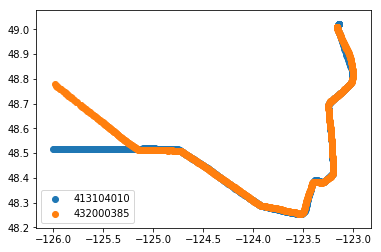
\includegraphics[scale = .8]{figures/VesselRendevouz2d}
\caption{Two vessel routes}
\label{fig: VesselRendevouz2d}
\end{figure}

While is obvious that the routes are similar in a positional way, they occur at different times, as is can be see in the figure ~\ref{fig: VesselRendevouz3d} .

\begin{figure}[H]
\centering
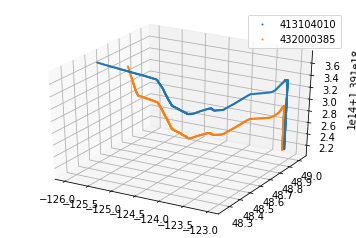
\includegraphics[scale = .9]{figures/VesselRendevouz3d}
\caption{Two vessel routes, time on Z-axis}
\label{fig: VesselRendevouz3d}
\end{figure}

%-----------RB-ADS-----------

\section{Rule Based Anomaly Detection Service}
\label{section: 4 Rule Based Anomaly Detection}
A Rule is defined as something that can, at least in the way we approach them, be expressed as an if-then sentence, \cite{Edlund2006RuleSea-Surveillance}
Anomaly Detection based on the definition of rules, is extremely used in the literature, as it represents an effective way to detect Anomalies at seas. Although this in only viable if and only if the rules are defined by Subject Matter Experts (SMEs) \cite{Boinepalli2014AAlgorithm, Will2011FastProcesses}.

Rule Based Anomaly Detection Service, was developed to detect Anomalies that can be codified into a rule or a set of rules, in real-time. 
Our approach to detect Anomalies in real-time was by storing the $N$ last Behavioural Points for each Vessel in a Service Cache, working like a first in first out (FIFO) queue. $N$ is a configurable Value, which represents the limit of messages stored in Service Cache for each Vessel, we provide an intuitively way to reduce the hardware requirements to run this service in Real-Time.

When the Service Cache has stored $N$ $BPs$ for a certain Vessel the Rule Based Anomaly Service is called for this Vessel, as demonstrated in Figure\ref{fig: RB-ADS}, in Vessel MMSI n case.
If a Vessel queue has $N$ $BPs$, and was the Rule Based Anomaly Service was already called of this messages, all Vessel Service Cache being FIFO, we discard the oldest $BPs$, thus the Vessel Queue after is full for the first time it as always $N$.

\begin{figure}[H]
\centering
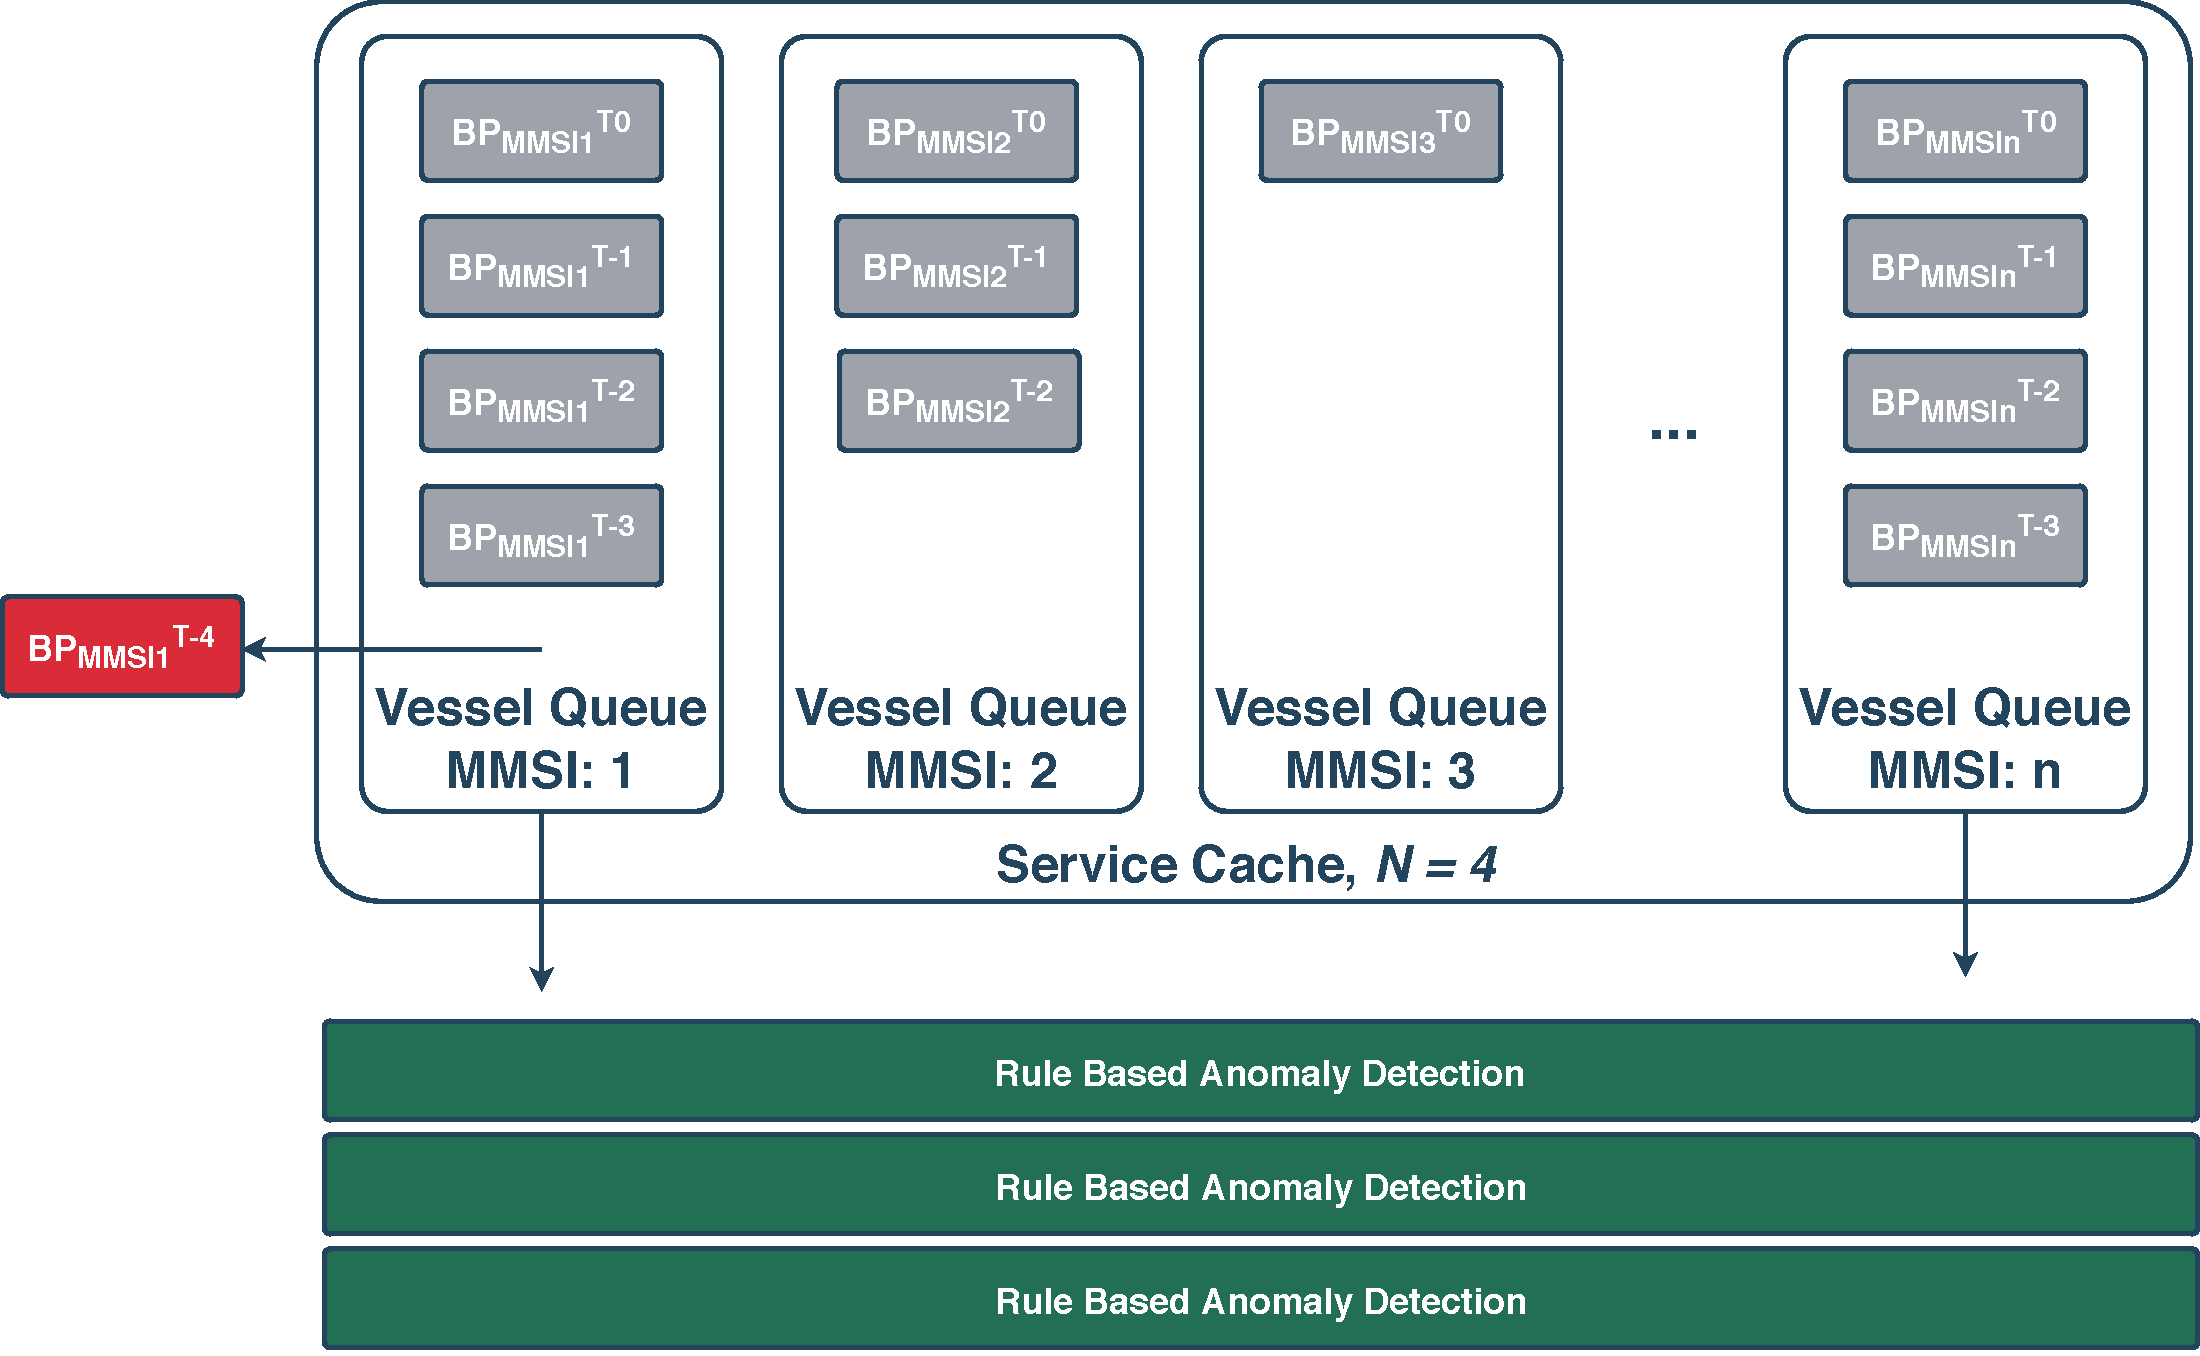
\includegraphics[scale = .36]{figures/Ch4/RB-ADS.pdf}
\caption{Demonstration of a possible cases for RB-ADS Service Cache coordinator.}
\label{fig: RB-ADS}
\end{figure}

Rule-Based Anomaly Detection Service, allows a detection of Anomalies based on little previous knowledge of each Vessel Trajectory. Despite the Service could be configured with any Rule that could be written for either Temporal, Spatial or Features based Rules, for example:

\textit{If Vessel MMSI: X in Zone: Y Stopped for more than M minutes then Report as Anomaly.}

For this work we decided to focus on the creation of configurable Rules that could detect the Anomalies presented in Section XX, as were the Anomalies that would be Validated by Maritime Officers,  which we present in Subsections Under.

\subsection{Speed}
\label{subsection: 4 Speed}
Speed represents a Set of configurable Rules that were implemented to detect the Anomaly, $(AR_2)$, defined in Section XX.

Our first approach for the detection of an \textit{Abnormal Change of Velocity} was, calculating the $SoG$ difference from the latest received, $BP^T$ with the previous $BPs^{T-1}$, stored in the Vessel Queue.
If the difference is bigger than a defined $SoG$ $Treshold$, then an Anomaly is generated with the $BPs$ stored in the Message Queue, and the configurations that generated this Anomaly, which could be represented as:
\begin{align*}
\mathbf{if}\;\;& abs({BP_{MMSIn}}^{T}.SoG - {BP_{MMSIn}}^{T-1}.SoG) > SpeedThreshhold
\;\;\mathbf{then} \\ 
&Anomaly[{BP_{MMSIn}}^{T}, {BP_{MMSIn}}^{T-1}] 
\end{align*}
Although, calculating the $SoG$ difference was only viable if  $N = 2 $ was considered as the size of the Vessel Queue.
When considering more than two $BPs$ the difference is not representative of the actual \textit{Abnormal Change of Speed}, in order to mitigate this we created a new configuration, representing the operation it should be done in this case, which for this anomaly we considered the Average Difference, the Max Difference.

\subsection{Course}
\label{subsection: 4 Course}
Similar the \textbf{Speed} defined above, Course represents a Set of configurable Rules implemented for the Anomaly detection, of $(AR_1)$, which is the \textit{Detection of Abnormal change of Direction}. 
Our approach for the detection of $(AR_1)$ was quite similar to the {Detection abnormal change of Velocity}. 
Although, we noticed depending how Vessels are Moored at port\footnote{http://marineinsight.com/marine-navigation/mooring-methods-ships/}  Vessels tend to swing, due to the Sea Currents, or just from the movement of other Vessels moving in Ports. This creates abrupt changes of $CoG$, which are not representative of the Anomaly Requirement $(AR_1)$.

In order to mitigate this problem, we defined other configurable condition, Minimum SoG Threshold. Thus, the representation of the configurable Set of rules for the detection of rule for the detection of $(AR_1)$, is :

\[ If\; abs(MQ_{T}.CoG - MQ_{T-1}.CoG)\;and\; MQ_T.SoG > S\; then\; Anonalous.\]

\subsection{AIS Signal Loss}
\label{subsection: 4 AIS Signal Loss}
The \textit{disappearance from sensor coverage for more than a configurable Time Period}, $(AR_3)$, can be caused for numerous reason as it is mentioned in Section XX. From a data stand point the disappearance from sensor coverage is represented as the loss of signal, or in other words, the non reception of AIS messages from this Vessel for more than $M$ Minutes.

In this work, we detect the loss of signal from Vessel, by analyzing when did a certain Vessel transmitted for the last time. This is done in real time, by the RB-ADS by one of two ways: the A priori way or the posteriori way.

First, as we store the Last $N$ $BPs$ for each Vessel that we received AIS messages from, in a the respective Message Queue from the Service Cache. By calculating the difference between the the last received ${BP_{MMSI}}^T$ to the ${BP_{MMSI}}^T-1$, we can know what was the elapsed time. Therefore, if this elapsed Time is bigger than a configurable Time $M$, this is reported as Anomaly. This method is considered a posteriori, as we are waiting for a new message to generate a Signal Loss Anomaly.

The a priori way, is when a Signal Loss anomaly is generated with out the reception of the a new message of a certain Vessel. Having the latest $BP$ for each Vessel stored in the Vessel Queue, if more than $M$ minutes have passed without receiving a Message for this Vessel an anomaly is generated. Both methods of detection represent the actual Signal Loss from a Data Stand point, and depending on the situation both can generate value to the End-Users. 

